% This file was created with tikzplotlib v0.10.1.
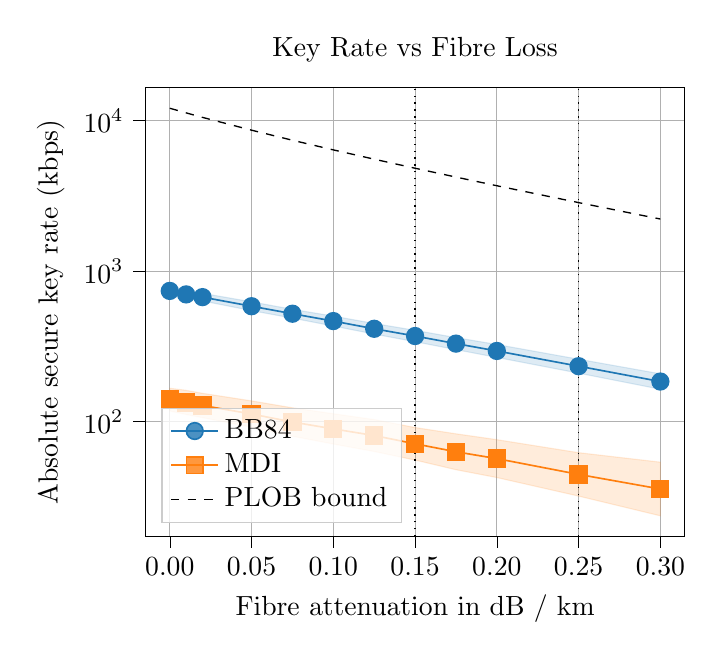
\begin{tikzpicture}
\definecolor{darkgray176}{RGB}{176,176,176}
\definecolor{darkorange25512714}{RGB}{255,127,14}
\definecolor{darkred}{RGB}{139,0,0}
\definecolor{lightgray204}{RGB}{204,204,204}
\definecolor{steelblue31119180}{RGB}{31,119,180}
\begin{axis}[
title={Key Rate vs Fibre Loss},
legend cell align={left},
legend style={
  fill opacity=0.8,
  draw opacity=1,
  text opacity=1,
  at={(0.03,0.03)},
  anchor=south west,
  draw=lightgray204
},
log basis y={10},
tick align=outside,
tick pos=left,
x grid style={darkgray176},
xlabel={Fibre attenuation in dB / km},
xmajorgrids,
xmin=-0.015, xmax=0.315,
xtick style={color=black},
xtick={-0.05,0,0.05,0.1,0.15,0.2,0.25,0.3,0.35},
xticklabels={
  \(\displaystyle {\ensuremath{-}0.05}\),
  \(\displaystyle {0.00}\),
  \(\displaystyle {0.05}\),
  \(\displaystyle {0.10}\),
  \(\displaystyle {0.15}\),
  \(\displaystyle {0.20}\),
  \(\displaystyle {0.25}\),
  \(\displaystyle {0.30}\),
  \(\displaystyle {0.35}\)
},
y grid style={darkgray176},
ylabel={Absolute secure key rate (kbps)},
ymajorgrids,
ymin=17.3005432522986, ymax=16535.2938160824,
ymode=log,
ytick style={color=black},
ytick={1,10,100,1000,10000,100000,1000000},
yticklabels={
  \(\displaystyle {10^{0}}\),
  \(\displaystyle {10^{1}}\),
  \(\displaystyle {10^{2}}\),
  \(\displaystyle {10^{3}}\),
  \(\displaystyle {10^{4}}\),
  \(\displaystyle {10^{5}}\),
  \(\displaystyle {10^{6}}\)
}
]
\path [draw=red, fill=red, opacity=0.08]
(axis cs:0.15,0)
--(axis cs:0.15,1)
--(axis cs:0.25,1)
--(axis cs:0.25,0)
--cycle;
\path [draw=steelblue31119180, fill=steelblue31119180, opacity=0.15]
(axis cs:0,781.466288525412)
--(axis cs:0,698.64309558436)
--(axis cs:0.01,661.40159698288)
--(axis cs:0.02,633.862062397348)
--(axis cs:0.05,546.692600663908)
--(axis cs:0.075,487.269170526123)
--(axis cs:0.1,431.770450590751)
--(axis cs:0.125,381.741745986002)
--(axis cs:0.15,339.606527531744)
--(axis cs:0.175,300.806786733639)
--(axis cs:0.2,267.045331522423)
--(axis cs:0.25,209.909891062134)
--(axis cs:0.3,164.059368211718)
--(axis cs:0.3,207.760566292931)
--(axis cs:0.3,207.760566292931)
--(axis cs:0.25,259.733664087754)
--(axis cs:0.2,325.402611391929)
--(axis cs:0.175,361.607495404389)
--(axis cs:0.15,404.188082279127)
--(axis cs:0.125,448.872867813999)
--(axis cs:0.1,502.329654145652)
--(axis cs:0.075,557.443156028326)
--(axis cs:0.05,625.223134459659)
--(axis cs:0.02,712.33963731441)
--(axis cs:0.01,742.460726530821)
--(axis cs:0,781.466288525412)
--cycle;
\path [draw=darkorange25512714, fill=darkorange25512714, opacity=0.15]
(axis cs:0,166.417508986879)
--(axis cs:0,117.688008626104)
--(axis cs:0.01,111.47332187609)
--(axis cs:0.02,106.24949667238)
--(axis cs:0.05,91.8939154960214)
--(axis cs:0.075,79.9807281625705)
--(axis cs:0.1,70.9648592947644)
--(axis cs:0.125,63.301939646205)
--(axis cs:0.15,55.488340751124)
--(axis cs:0.175,47.8648787203127)
--(axis cs:0.2,42.4591844955816)
--(axis cs:0.25,31.9665046691029)
--(axis cs:0.3,23.6336224866717)
--(axis cs:0.3,53.715077974749)
--(axis cs:0.3,53.715077974749)
--(axis cs:0.25,62.1057173558714)
--(axis cs:0.2,75.8110047746654)
--(axis cs:0.175,82.8994102236531)
--(axis cs:0.15,91.2623200092868)
--(axis cs:0.125,103.062941403529)
--(axis cs:0.1,112.69308742205)
--(axis cs:0.075,123.408782708677)
--(axis cs:0.05,137.228403602466)
--(axis cs:0.02,154.113643332818)
--(axis cs:0.01,161.286048224802)
--(axis cs:0,166.417508986879)
--cycle;
\addplot [semithick, steelblue31119180, mark=*, mark size=3, mark options={solid}]
table {%
0 738.895139319656
0.01 700.760094629078
0.02 671.956153060221
0.05 584.640796877015
0.075 521.17642334759
0.1 465.715686997512
0.125 413.948683154156
0.15 370.492794926607
0.175 329.809018602271
0.2 294.783392065123
0.25 233.496606257627
0.3 184.621415998597
};
\addlegendentry{BB84}
\addplot [semithick, darkorange25512714, mark=square*, mark size=3, mark options={solid}]
table {%
0 139.947651760159
0.01 134.086134883089
0.02 127.962873656614
0.05 112.296283662011
0.075 99.3495057999609
0.1 89.4273397367849
0.125 80.7718026076338
0.15 71.1617503326993
0.175 62.991826583618
0.2 56.7351164493644
0.25 44.5567357852261
0.3 35.6297891475287
};
\addlegendentry{MDI}
\addplot [line width=0.48pt, black, dotted, forget plot]
table {%
0.15 17.3005432522986
0.15 16535.2938160824
};
\addplot [line width=0.48pt, black, dotted, forget plot]
table {%
0.25 17.3005432522986
0.25 16535.2938160824
};
\addplot [line width=0.48pt, black, dashed]
table {%
0 12104.3469326774
0.01 11275.3723696512
0.02 10525.8352634677
0.05 8653.0199226264
0.075 7418.19360900341
0.1 6400.21138301092
0.125 5549.76915098966
0.15 4831.88038379219
0.175 4220.84384074114
0.2 3697.24598438335
0.25 2855.54193398454
0.3 2220.27636632398
};
\addlegendentry{PLOB bound}
\draw (axis cs:0.2,0.97) node[
  scale=0.35,
  anchor=north,
  text=darkred,
  rotate=0.0
]{\itshape Realistic hardware regime (Corning SMF-28)};
\end{axis}
\end{tikzpicture}
